\section*{Cache Model}~\par
	The initial phase of analysis is the construction of a model of classical control units as caches for quantum programs. Conceptually, quantum programs are compiled and scheduled with the ScaffCC framework which results in discretization of the programs into modules. Each of the modules compiled such that they self contained, and have no dependencies upon other modules with potential exceptions at module boundaries. The largest uncompressed module size provides a lower bound on the size of the cache memory.\par
	Simulations are performed on a per-program basis. The modules of each program are extracted, and unique binary codes are assigned to individual instructions, quantum register names, as well as module calls themselves. Once each module is converted to binary, each is compressed and decompressed across a series of different compression algorithms, and statistics regarding CPU usage and memory usage are collected with respect to each module. A program call stack is then simulated on control units of varying capacities (parameterized by number of containable modules), and total CPU usage required by decompression of modules is tracked. These statistics are then compared against the overall program runtime to determine significance of the decompression actions. Examples of these simulations are provided in (figure \ref{fig:ising}) and (figure \ref{fig:bwt}).\par 
	
\section*{Initial Results}
	Provided here are examples of the first stage statistics. The first set of plots depict the total CPU usage requirements for two different quantum programs, Ising Model and Binary Welded Tree. As can be seen, the CPU usage depends highly on the structure of the program module sizes.\par
\begin{figure}[h]
	\begin{minipage}{0.5\textwidth}
		\centering
		\includegraphics[width=\linewidth]{Figures/ising.png}
		\caption{Ising Model}
        \label{fig:ising}
	\end{minipage}\hfill
	\begin{minipage}{0.45\textwidth}
		\centering
        \includegraphics[width=1.1\linewidth]{Figures/bwt.png}
		\caption{Binary Welded Tree}
        \label{fig:bwt}
	\end{minipage}
\end{figure}

	The next analysis compares the CPU usage-padded runtimes against original program runtimes. Provided are two plots, the former (figure \ref{fig:full}) of the new program slowdowns due to decompressions, and the latter (figure \ref{fig:fullfocus}) a scaled view of the same plot. Slowdowns shown here are considerable, higher than 100x for many benchmarks. \par 
\begin{figure}[h]
	\begin{minipage}{0.5\textwidth}
		\centering
		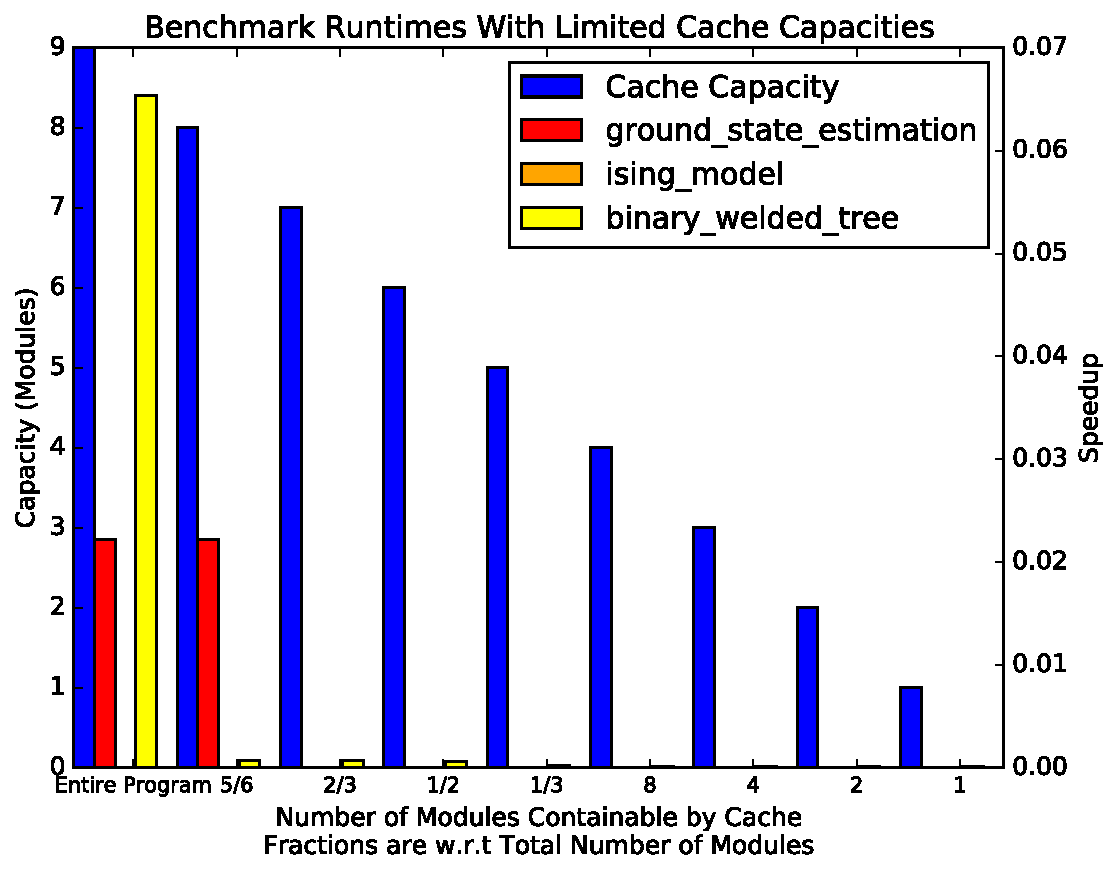
\includegraphics[width=\linewidth]{Figures/full.pdf}
		\caption{New Program Runtimes with Decompressions}
        \label{fig:full}
	\end{minipage}\hfill
	\begin{minipage}{0.45\textwidth}
		\centering
        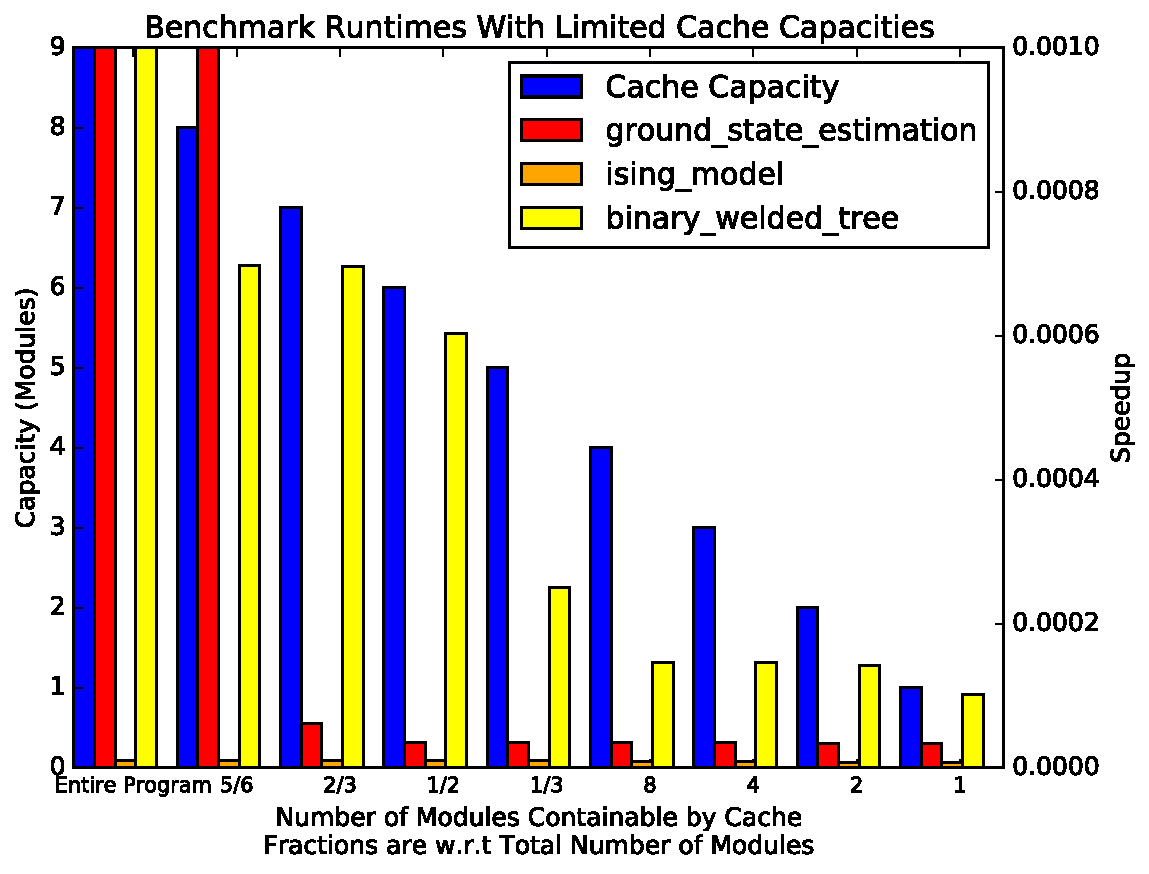
\includegraphics[width=1.1\linewidth]{Figures/fullfocused.pdf}
		\caption{Scaled Depiction of New Program Runtimes}
        \label{fig:fullfocus}
	\end{minipage}
\end{figure}

This initial analysis is intended to motivate the idea that restricting the memory sizes of control units has a dramatic effect on the runtimes of quantum programs, with dependence upon the internal structure of the program and distribution of module sizes.
